\documentclass[12pt]{article}

\usepackage{url} % websites in bib
\usepackage{hyperref}
\usepackage[a4paper,left=1in,right=1in,top=1in,bottom=1in]{geometry} % margins

\usepackage{amsmath}
\usepackage{amssymb}
\usepackage{commath}

\usepackage{todonotes}
\usepackage{float} % figure placement
\usepackage[]{algorithm2e}

\begin{document}
	\title{A benchmark for histogram building algorithms of numeric streams}
	\author{Stefan Sebastian, 242}
	\date{}
	\maketitle
	
	\newpage
	\tableofcontents
	\newpage

	\section{Introduction}
	The main goal of this paper is to provide a benchmark for algorithms 
	that build histograms over continuous streams of numeric data. 
	The main goals of the benchmark is to measure both performance 
	and accuracy in conditions resembling real streams of data: large 
	volumes, varying data distribution, concurrent additions and queries.
	The benchmark is implemented as a separate application which generates 
	data and communicates with the histogram clients using Kafka streams 
	and http requests for queries. It is applied over two algorithms taken
	from practical industry-tested environments: the Numeric Histogram\cite{HiveImplementation} from 
	the Apache Hive project and the Optimal Streaming Histogram from the Amplitude's 
	company blog\cite{OSHistograms}. The algorithms provide different approaches 
	to solving the main issues of stream bucketing algorithms, enuntiated above, 
	however, after being put through the benchmark they seem to behave very similarly
	in terms of execution times and approximation error.
	
	\subsection{Histograms}
	A histogram is a type of plot that shows the underlying distirbution of a set of 
	data\cite{DataStreamsHistograms}. In this paper the actual meaning of the term is the data structure out of 
	which this plot can be built. An example of such a plot can be seen in figure \ref{histogram}.
	The main use of such methods is to provide a quick and easy to interpret summary 
	of the data, which can then be analyzed by a domain expert to aid in various 
	business decisions. The supporting data structure can also be used by other 
	more complex algorithms. For example, Bel-Haim et al.\cite{Ben-Haim:2010:SPD:1756006.1756034}
	proposed an algorithm for classification of streaming data which leverages histograms 
	for obtaining a light weight summary of the incoming data.
	
	Most algorithms and mehtods for building histograms are thought out with the presumption 
	that the data set is known in advance and has a reasonable size. 
	However, this does not hold in the case of data 
	streams, where data is accumulated over time in huge volumes, 
	which causes a number of issues for the classic algorithms. First of all, 
	the size of the data can be gigantic, meaning that it is not reasonable to 
	store each point and its occurences, and an approximation heuristic is required.
	Furthermore, the distribution of the data is unknown beforehand, and this 
	can cause issues if we can't properly store incoming data. Given the limitation
	of the first point, the algorithm needs to keep a limited number of buckets, but these 
	must not be fixed in the beginning because the values represented by the buckets might not
	be relevant if the distribution of the data changes over time. Finally, these algorithms 
	must be able to absorb data and perform queries constantly, meaning that performance is 
	also an important factor.

	A mathematical model for this data structure can be described as: a set of B pairs (called bins)
	of the form ${(p_1, m_1), .., (p_B, m_B)}$. The value of the m variables represent the number 
	of points observed for the p variables. The meaning of the p variables depends upon the bucketing 
	algorithm. For example, in the Ben-Haim's algorithm\cite{Ben-Haim:2010:SPD:1756006.1756034},
	p represents a central point for the interval and m the number of values around it. In the 
	second algorithm discussed in the paper $p_i$ represents the lower bound of the considered interval,
	with the upper bound being the the value of $p_{i+1}$.
	
	\begin{figure}[H]
		\label{histogram}
		\caption{Example of a histogram showing the frequency of age data\cite{HistogramExample}}
		\centering
		  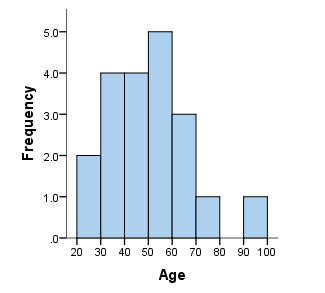
\includegraphics[width=0.5\textwidth]{histogram.png}
	\end{figure}

	\subsection{Motivation}
	The field of data streams has been evolving at a very fast rate in order 
	to match the explosion in continuous sources of data: user activity logs,
	web application metrics, sensor data from various domains like traffic or 
	healthcare \cite{DataStreams}. Given this recent development, a lot of 
	algorithms that were designed for batch processing do not perform so well 
	in a streaming environment. A class of such algorithms are the ones used 
	to build histogram models. There is little research in this domain which 
	causes developers to come out with their own in-house methods for the task.
	This article aims to contribute to the development of the field, to 
	provide a comparison of the currently available algorithms and a baseline 
	with which to compare future stream histogram methods.  

	\subsection{Paper outline}
	The paper is organized in four main chapters. The first, contains an introduction 
	into the topic and summarizes the goals of the experiment. The second chapter 
	describes the algorithms which were put under the benchmark, providing snippets 
	of implementation and covering advantages and disadvantages. The next chapter 
	covers the benchmarking client, the methodology and the test results. Finally,
	the conclusion provides a short overview of the experiment and final results.

	\section{Algorithms}
	\subsection{Numeric Histogram}
	\subsubsection{Overview}
	The Numeric Histogram algorithm first appeared in the paper by Ben-Haim and Tom-Tov
	on building a streaming parallel decision tree algorithm\cite{Ben-Haim:2010:SPD:1756006.1756034}.
	The main focus was to describe a method for tree based classifiers for large data 
	sets in a distributed environment, however they needed a data structure that 
	can summarize large amounts of data accurately. Thus, they proposed a histogram 
	data structure that can adapt to the requirements of a streaming environment. 

	The histogram maintains a fixed number of bins of the shape (p, m) where 
	p represents a central value of the interval and m the number of points in it.
	Initially the histogram has some bins allocated but the values are not known. 
	They are filled as data comes is added into the structure and once the allocated 
	number of bins is reached the central bin values are updated depending on incoming
	values. In this regard, the algorithm is robust to changes in data patterns over 
	a longer period of time, which is one of the main concerns of streaming analysis 
	algorithms.

	\subsubsection{Procedures}
	The proposed data structure contains four procedures: update, merge, sum and uniform.
	But for the purpose of this benchmark only two were needed: update and sum. The update 
	procedure adds a new point to the histogram data structure and is described in algorithm \ref{add}.

	\begin{algorithm}
		\label{add}
		\KwData{histogram $h = {(p_1, m_1), .., (p_b, m_b)}$, a point p}
		\KwResult{a histogram that represents the set $S \bigcup \{p\}$}
		binary search for the closest $p_i$ larger than p\;
		\eIf{$p_i = p$}{
			$m_i = m_i + 1$\;
		}{
			add a new bin of shape (p, 1) to the histogram at the i-th position\;
			find the closest two bins by their p values\;
			merge those bins, moving p proportional to their m values\;  
		}
		\caption{add procedure}
	\end{algorithm}

	The sum procedure, depicted in algorithm \ref{sum}, obtains the estimated number of points between $(-\infty, n]$ where n is 
	the input value. In order to estimate the number of values in a range $[a, b]$ we can calculate 
	$sum(b) - sum(a)$. The algorithm assumes that for each bin (p, m), there are $m/2$ points to the left of p
	and $m/2$ to the right. This means that the number of points in the interval $[p_i, i_{i+1}]$ is equal 
	to $(m_i + m_{i+1}) / 2$, which is the area of the trapezoid $(p_i, 0), (p_i, m_i), (p_{i+1}, m_{i+1}), (p_{i+1}, 0)$, 
	divided by $p_{i+1} - p_i$. Similarly, we can estimate the number of points in the 
	interval $[p_i, p]$ by adding calculating its projection on the line from $(p_i, m_i)$ to
	$(p_{i+1}, m_{i+1})$, then find the area of the new trapezoid and dividing again by $p_{i+1} - p_i$.
	The algorithm will not work properly if the point p is smaller than $p_0$ or larger than 
	$p_b$. For this reason the data structure should be initialized with a lower and upper bound
	into which all incoming data should fit.

	\begin{algorithm}
		\label{sum}
		\KwData{a histogram h, a point p such that $p_1 < p < p_b$}
		\KwResult{estimated number of points in the interval $[-\infty, p]$}

		binary search to find i such that $p_i <= p <= p_{i+1}$\;
		set $s = (m_i + m_p) \cdot (b - p_i) / 2 \cdot (p_{i+1} - p_i) $\;
		where $m_p = m_i + (m_{i+1} - m_i) \cdot (p - p_i) / (p_{i+1} - p_i)$\;

		\For{$j < i$}{
			$s = s + m_j$\;
		}
		$s = s + m_i / 2$\;
		\caption{sum procedure}
	\end{algorithm}

	\subsubsection{In practice}
	This algorithm was adapted and implemented into the open source project Apache 
	Hive\cite{Thusoo:2009:HWS:1687553.1687609}, which is a datawarehouse solution 
	built on top of Hadoop to provide data query and analysis methods. The project 
	is used actively in industry, handling reporting tasks for large volumes of data,
	for e.g. data produced by 435M monthly users of Chitika\cite{HivePoweredBy}.
	The version of the algorithm presented in this report is based on the Hive 
	implementation, called NumericHistogram\cite{HiveImplementation}. The optimal 
	number of bins is left as a choice to the user, however the suggested range 
	is between 20 and 80.

	The algorithm is adaptable and can work with any ranges of data, however 
	the access to its underlying structure must be synchronized which 
	slows down execution in case of concurrent queries and insertions.

	\subsection{Optimal Streaming Histograms}
	\subsubsection{Overview}
	This algorithm was presented in a blog post\cite{OSHistograms} 
	by an engineer from the Amplitude company. Therefore, it was developed 
	with industry requirements in mind, and tested in realistic conditions 
	before being published. The main challenge was to avoid storing gigantic 
	amounts of streaming data and to uncover an optimal bucketing solution.
	The key requirements they identified for the bucket boundaries were:
	to be useful and reasonable for any range of data and to remain 
	useful upon changes in data distribution.
	
	The algorithm was also designed with data visualization needs in mind. 
	For this reason the buckets size and spacing have been thought out to 
	look intuitive in a chart and be easy to interpret.

	\subsubsection{Iterations}
	In order to reach a satisfying solution they went through multiple iterations 
	of the algorithm. The first one was to save the first 1000 distinct values 
	on the stream and then make evenly spaced buckets using them. However, this 
	method behaves poorly when distribution changes over time because the buckets 
	are fixed. Also, this might have resolution issues when the distribution 
	is skewed, for example: a lot of points in a small range of values. 
	
	The second technique was iterative merging of the closest values into buckets. 
	This was done in order to solve the resolution problem. Basically, among the 
	first 1000 values, the 2 closest ones are merged into a bucket. This process 
	is repeated until only 50 buckets are left. This improves resolution, however 
	it causes difficulties in interpreting the histograms as all buckets have 
	different widths and the spacing seems arbitrary. 

	\subsubsection{Algorithm}
	The final form of the algorithm is to pre-create buckets on a logarithmic 
	scale. This requires the user to know the boundaries of the incoming data, 
	and then, using those bounds, to create buckets that have 10\% increments 
	for every order of magnitude. For example, for the range 1 - 10, there will be 
	buckets of size 0.1, for the range 10 - 100, of size 1 and so forth. This solves
	the resolution issues because each value will be in a bucket in a 10\% range 
	of its true value. The spacing issues are also solved, and data visualization
	is easier and more intuitive. The fixed size of the buckets should not be a 
	problem in this scheme, which should work with a variety of data set types.

	\subsubsection{Implementation}
	The blog post did not provide an implementation so a variant will be 
	proposed in this report. The initialization step is done with a given 
	lower and upper bound. The smallest power of 10 larger than the upper bound 
	and the largest power of 10 smaller than the lower bound are found and 
	for each value p between them 90 buckets of width $p / 10$ are created.

	For the add procedure, the bucket is found using binary search which 
	provides a logarithmic complexity. The bin is the incremented by 1 
	for each addition. In order to estimate\ref{estimateOSH} the number of values in a range $ [a, b] $ 
	two binary searches are performed, for the bin of a and the bin of b. We 
	need to estimate the number of values in the range $[a, bUb]$, where bUb is the upper
	bound of the bucket which contains a, and in the range $[bLb, b]$ where bLb is the
	lower bound of the bucket which contains b. The approach is similar for both 
	intervals, so only one will be described. In order to estimate the number 
	of values in $[a, bUb]$, a ratio is calculated between the distance from 
	a to the upper bound and the size of the bucket. This ratio is then multiplied 
	with the number of values in the bucket. The values for the buckets contained 
	in the range $ [bUb, bLb] $ are added as they are.
	
	\begin{algorithm}[H]
		\label{estimateOSH}
		\KwData{a histogram h, two points a, b}
		\KwResult{estimated number of points in the interval $[a, b]$}

		estimate = 0\;
		bin1 = getBin(a), bin2 = getBin(b)\;
		$lowerBound = bin1.val$, $upperBound = lowerBound \cdot 10$\;
		$ratio = (upperBound - a) / (upperBound - lowerBound)$\;
		$estimate = estimate + ratio \cdot bin1.count$\;

		\For{each bin from bin1 to bin2} {
			$estimate = estimate + bin.count$
		}

		$lowerBound = bin2.val$, $upperBound = lowerBound \cdot 10$\;
		$ratio = (b - lowerbound) / (upperBound - lowerBound)$\;
		$estimate = estimate + ratio \cdot bin2.count$\;

		\caption{Estimated number of points in range}
	\end{algorithm}

	\subsubsection{Remarks}
	In the current iteration this algorithm has some weak points. The main 
	issue is that buckets are fixed before execution, which means that 
	the building algorithm should be adapted to incoming data. For example, 
	the algorithm currently does not support negative numbers and performs 
	poorly for small ranges of very large values as illustrated in the benchmark.
	
	\section{Benchmark}
	This paper proposes a benchmark for histogram building algorithms 
	over continuous data streams. The benchmark aims to address some 
	issues which are specific to these types of problems: a large amount 
	of data, which is usually not practical to store, varying distribution 
	of data, meaning the algorithms must adapt to changes and have an 
	efficient bucketing algorithm, and the mixing of input and queries from 
	multiple channels, which means an ideal algorithm would have little overhead 
	for doing multiple operations concurrently.

	\subsection{Metrics}
	The benchmark contains several test suites which attempt to cover all these 
	situations. It is run as a separate application which communicates with 
	the histogram building applications through a stream of data to be added, 
	and a list of queries over the input data. The metrics measured are: average 
	request time, mean squared error and mean absolute error.

	Average request time represents the cumulated execution time of all queries 
	divided with the number of queries. The time is measured by the benchmarking 
	application from the moment the query request is sent to the moment the answer 
	is received. This metric aims to measure algorithm performance and might 
	also indicate issues with concurrency, caused by attempting to perform 
	queries while the algorithm also performs additions from the input stream.
	
	Mean absolute error\cite{errormetrics} is defined as $ MAE = \frac{1}{n} \cdot \sum \abs{y - \hat{y}} $
	and it's one of the simplest regression metrics. It calculates the residual for 
	every query result compared to actual expected answer and takes the absolute 
	value so that positive and negative values don't cancel each other out.

	Mean squared error\cite{errormetrics} can be calculated as $ MSE = \frac{1}{n}
	\sum (y - \hat{y})^2 $. It is similar to MAE, however it instead squares the difference.
	The main consequence of squaring the difference is that MSE is more sensitive 
	to outliers in the results, because the error grows quadratically. Thus, the model 
	is punished more if it makes predictions which are far from the expected value.

	\subsection{Implementation}
	For this benchmark two histogram algorithms with proven practical results 
	were implemented in the Java programming language using the libraries 
	provided by the Spring Boot framework. 
	The aforementioned algorithms are the Numeric Histogram\cite{HiveImplementation} 
	from the Hive project and Optimal Streaming Histogram\cite{OSHistograms} developed 
	by software engineers from Amplitude. The algorithms are contained in a standalone 
	application which provides two input channels: a HTTP Rest API and a Kafka reader.

	The application API exposes methods for initializing the bucketing algorithms, 
	which requires the expected range into which the data will fall, and methods 
	for queries. A query is of the type 'approximately how many points were observed
	in the given range?' and in realistic scenarios they are used for statistics 
	and data mining processes started by users and don't come into the application 
	as a continuous stream. Apache Kafka\cite{Kafka} is a distributed streaming platform
	used for building real time data pipelines with strong fault-tolerance guarantees.
	This message queue was selected to model incoming data streams, which, in this 
	case represent values to be added into the histogram.

	The benchmarking component runs as a separate Spring Boot application which 
	exposes an API that starts the different available benchmarks. The user 
	can provide some parameters: which benchmark to perform, how many operations, 
	what's the ratio of queries to additions, and which are the bounds of the data that is 
	generated. An overlook of the architecture is given in figure \ref{architecture}.
	The entry point is the BenchmarkController which reads from the user a list of 
	parameters, contained in the stats class. The actual work is done by the BenchmarkEngine
	which generates a list of actions, executes them, records response times and query values 
	and then generates a report for each algorithm in the system. Input data for the 
	histogram algorithms is sent through a Kafka queue, on a different topic for each 
	algorithm.

	\begin{figure}
		\label{architecture}
		\caption{Architectural diagram of the benchmarking application}
		\centering
		  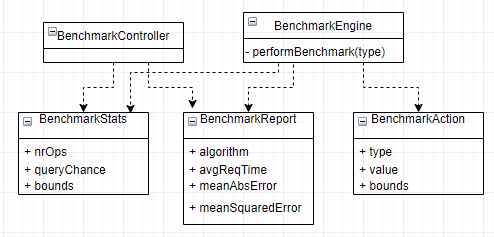
\includegraphics[width=0.8\textwidth]{diagram.png}
	\end{figure}

	\subsection{Tests and results}
	The benchmark contains tests that can be divided into two main categories:
	for performance and for accuracy. The accuracy tests are designed to cover 
	some distribution which might appear over time on a data stream. The first 
	such distribution is uniform, which 
	is the simplest one and should not cause any issues. A second test in this 
	category is with a skewed distribution, where the first 80\% of operations 
	cover the first 20\% of the value range and the rest 20\% of the operations 
	cover the remaining range. A third scenario for the value range to change 
	twice at a third and two thirds of the testing interval. These last two scenarios 
	are designed to test the ability of the algorithm to adapt to changes in 
	the distribution of the incoming data stream.

	The performance oriented tests are focused on testing the system under 
	a lot of queries, which tends to be the most costly operation. Another 
	situation is with a large range of possible data values, which means 
	that in case of dynamic bucketing, the values might have to change 
	more often as the chance of the same value arriving multiple times is 
	reduced.

	A special test case was designed to point out a weakness of the 
	OptimalStreamingHistogram in its current form, which uses a small 
	range of large values (1000000, 1000100).

	\begin{table}[h!]
		\begin{center}
		  \caption{Uniform distribution; 1mil operations, 1\% of them queries, bounds (0, 100)}
		  \label{tab:uniform}
		  \begin{tabular}{c|c|c|c}
			\textbf{Algorithm} & \textbf{Avg Req Time} & \textbf{MAE} & \textbf{MSE}\\
			\hline
			NumericHistogram & 3.09 & 161536 & 52098973486 \\
			OptimalStreamingHistogram & 3.14 & 161624 & 52131831979 \\			
		  \end{tabular}
	    \end{center}
    \end{table}


	\begin{table}[h!]
		\begin{center}
			\caption{Skewed distribution; 1mil operations, 1\% of them queries, bounds (0, 100)}
			\label{tab:uniform}
			\begin{tabular}{c|c|c|c} 
				\textbf{Algorithm} & \textbf{Avg Req Time} & \textbf{MAE} & \textbf{MSE}\\
				\hline
				NumericHistogram & 6.30 & 102856 & 23614668551 \\
				OptimalStreamingHistogram & 4.81 & 103477 & 23626580730 \\
			\end{tabular}
		\end{center}
	\end{table}
			
	\begin{table}[h!]
		\begin{center}
			\caption{Twice changing distribution; 1mil operations, 1\% of them queries, bounds (0, 100)}
			\label{tab:uniform}
			\begin{tabular}{c|c|c|c}
				\textbf{Algorithm} & \textbf{Avg Req Time} & \textbf{MAE} & \textbf{MSE}\\
				\hline
				NumericHistogram & 3.45 & 52115 & 5385128831 \\
				OptimalStreamingHistogram & 3.13 & 51968 & 5344437433 \\
		  \end{tabular}
		\end{center}
	\end{table}

	\begin{table}[h!]
		\begin{center}
			\caption{Uniform distribution; 1mil operations, 1\% of them queries, bounds (0, 100000)}
			\label{tab:uniform}
			\begin{tabular}{c|c|c|c}
				\textbf{Algorithm} & \textbf{Avg Req Time} & \textbf{MAE} & \textbf{MSE}\\
				\hline
				NumericHistogram & 3.44 & 166381 & 54802576827 \\
				OptimalStreamingHistogram & 3.03 & 166345 & 54665682814 \\
		  \end{tabular}
		\end{center}
	\end{table}

	\begin{table}[h!]
		\begin{center}
			\caption{Uniform distribution; 1mil operations, 90\% of them queries, bounds (0, 100)}
			\label{tab:uniform}
			\begin{tabular}{c|c|c|c}
				\textbf{Algorithm} & \textbf{Avg Req Time} & \textbf{MAE} & \textbf{MSE}\\
				\hline
				NumericHistogram & 3.37 & 16356 & 535437528 \\
				OptimalStreamingHistogram & 2.83 & 16350 & 534797489 \\
		  \end{tabular}
		\end{center}
	\end{table}

	\begin{table}[h!]
		\begin{center}
			\caption{Uniform distribution; 1mil operations, 1\% of them queries, bounds (1000000, 1000100)}
			\label{tab:uniform}
			\begin{tabular}{c|c|c|c}
				\textbf{Algorithm} & \textbf{Avg Req Time} & \textbf{MAE} & \textbf{MSE}\\
				\hline
				NumericHistogram & 3.39 & 160078 & 50782133935 \\
				OptimalStreamingHistogram & 3.04 & 491258 & 321320234951 \\
		  \end{tabular}
		\end{center}
	\end{table}

	We can observe that both algorithms behave surprinsingly similar in all test cases. 
	The average response time seems to be very close for all tests, at around 3 milliseconds for 
	tests which consider 1 million elements, with NumericHistogram being just a bit slower.	
	An exception is the skewed distribution test case where OptimalStreamingHistogram is 
	around 2 milliseconds faster than the other algorithm.
	
	The last scenario points out the weakness of the OptimalStreamingHistogram,
	which lies in the way the buckets are built. For a small range of large 
	values most of them fall into the same bucket, which causes the algorithm 
	to give inaccurate responses. It can be seen that the error is around 3 
	times larger than that of the NumericHistogram algorithm.

	\section{Conclusions}
	The main goal of creating a benchmark for various scenarios of data stream 
	bucketing was achieved. The benchmark was executed for two popular algorithms 
	in the field and uncovered the fact that they behave very similar. A noticeable 
	difference is when using large values, which causes the OptimalStreamingHistogram algorithm 
	to give out inaccurate responses. In terms of speed NumericHistogram seems to 
	be slightly slower than the other algorithm.

	\newpage
	\bibliography{references}
	\bibliographystyle{ieeetr}
\end{document}